\documentclass[a4paper]{article}
\usepackage{graphicx}
\usepackage{listings}
\usepackage[utf8]{inputenc}
\usepackage{caption}

\title{Trabajo Práctico Nro. 3:\\``Sistema de llenado\\y vaciado de un tanque''}
\author{Amodey, Leandro - leandroamodey@gmail.com
\and Monti, Matías - matiasmonti@hotmail.com
\and Quinteros, Fernando - lordfers@gmail.com
\and Araneda, Alejandro – eloscurodeefeso@hotmail.com}
\date{1er. Cuatrimestre 2020\\Jueves, 25 de Junio}

\def\teacher{Ing. Jorge H. Doorn
\and Ing. Matías Presso}

\captionsetup{justification=centering,labelsep=period,font={small},%
labelfont=bf,textfont=it}
\renewcommand{\figurename}{Figura}
\renewcommand{\abstractname}{Resumen}
\renewcommand{\refname}{Referencias}
\let\originalcite\cite
\renewcommand{\cite}[2][]{\textsuperscript{\originalcite{#2}}}
\makeatletter\let\@afterindentfalse\@afterindenttrue\makeatother
\let\originalappendix\appendix
\renewcommand{\appendix}{%
    \newpage\originalappendix\pagenumbering{gobble}%
    \renewcommand\thesection{Anexo \Alph{section}}
    \setcounter{secnumdepth}{1}
}
\setcounter{secnumdepth}{0}

\begin{document}

\begin{titlepage}\renewcommand\and\par\centering\makeatletter
    
\includegraphics{logo.png}\par
    {\Large Ingeniería en Computación \par}\vspace{0.5cm}
    {\LARGE Laboratorio de Microprocesadores \par}\vfill
    {\huge \@title \par}\vfill
    Grupo 2:\par
    \@author\vfill
    Práctica entregada:\par
    \@date\vfill
    Docentes:\par
    \teacher\vspace{1cm}\makeatother
\end{titlepage}

\begin{abstract}

    En el presente trabajo realizamos el análisis y diseño de la
    implementacion de un sistema que se ocupa del llenado y vaciado 
    de un tanque mediante el uso de microcontroladores y otros 
    componentes electrónicos.

\end{abstract}

\section{Introducción}

\section{Descripción de la Práctica}

\subsection{Enunciado}

A continuación transcribimos el enunciado original de la práctica del
que se extraen los requerimientos para el desarrollo.

\begin{quotation}

    \begin{center}\textit{\textbf{%
        Taller de Microprocesadores: Trabajo Practico N° 3%
    }}\end{center}\vspace{1em}

    Diseñar un sistema que permita llenar y vaciar un tanque de líquido 
    con dos bombas independientes. 

    El inicio de llenado del tanque debe realizarlo mediante un botón 
    (o señal digital externa ) y deben ingresar 500 lts (o cierto volumen 
    fijo). El vaciado también puede realizarse con un botón o señal 
    digital externa. El llenado no puede realizarse si el tanque esta por 
    encima de cierto nivel, y el vaciado deber finalizar con un nivel 
    mínimo en el tanque para proteger que la bomba no funcione sin 
    líquido. El vaciado no puede en caso que no existe ese nivel mínimo y 
    debe indicarse con una luz que el tanque se encuentra en su mínimo 
    nivel.

\end{quotation}

\subsection{Plataforma de Desarrollo}

El microcontrolador es programado utilizando el lenguaje C. 
Presentamos como anexo una copia del código fuente.

El \textit{firmware} que se implanta en el microcontrolador es  
producido con el compilador MPLAB XC8\cite{bib:compilador} de la 
empresa Microchips, diseñado específicamente para la línea de 
microcontroladores de 8 bits a la que pertenece el PIC12F675.

El diseño y simulación del esquemático correspondiente se realiza 
con el software Proteus\cite{bib:simulador} de la compañía 
Labcenter Electronics.

\subsection{Instrucciones de Compilación y Ejecución}

Para la compilación del firmware utilizamos la línea de comandos en 
una terminal. Como parámetro a la ejecución del compilador agregamos
el modelo del microcontrolador donde se instala el software. Éste es 
el método recomendado por el desarrollador por sobre el de incluir en 
el código mismo los archivos de encabezado para el preprocesador con 
las configuraciones específicas del modelo. Por ejemplo, para el 
primer ejercicio utilizamos:

\begin{center}\ttfamily 
	xc8 --chip=12f675 ejercicio1.c
\end{center}

El compilador genera un archivo {\ttfamily .hex} que es el que
agregamos a las propieda-des del microcontrolador solicitadas 
por el software Proteus para la simulación del circuito. Allí también 
indicamos tanto la frecuencia del reloj y la palabra que representa 
los bits de configuración que debieran ser impresos en la memoria del
integrado junto con el código ejecutable. 

\section{Diseño del sistema}

    \subsection{Caso de uso}

    Completar

    \subsection{Diagrama de arquitectura}

    Completar

    % --- Para insertar una imagen escriban de acá
    \begin{figure}[h]\centering
    % La opcion `[h]` es para "here", pero puede cagarse en eso.
    % No usar "la imagen que sigue" sino la referencia.
        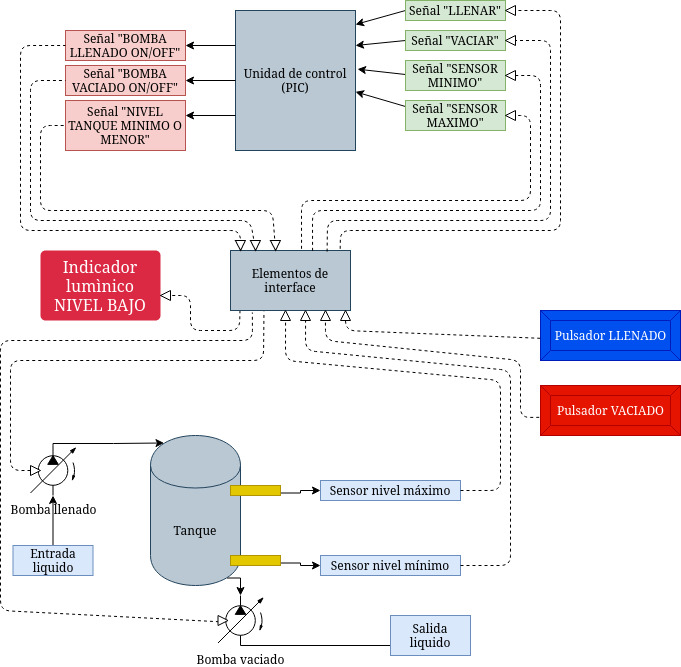
\includegraphics[height=12cm]{diagrama_sistema.jpg}
        \caption{Esquema del sistema general.}\label{fig:esquematico1}
    \end{figure}
    % --- hasta acá.

    \subsection{Esquemático del circuito.}

    \subsection{Descripción de funcionamiento.}



    
\section{Análisis y simulación.}

\subsection{Completar las subsecciones}

\section{Conclusiones}

Completar

\noindent\rule{\textwidth}{1pt}
% Linea horizontal sin identacion y del ancho del texto

\begin{thebibliography}{9}
% Comienza la bibliografia
% El "9" indica que el espacio para imprimir "9" es de la mayor referencia

% Para agregar una entrada a la bibliografia repetir de aca
\bibitem{bib:boylestad} 
Boylestad, R. \& Nashelsky, L. (2002). 
\textit{``Electronic devices and circuit theory"}.
Upper Saddle River, N.J: Prentice Hall.
% Hasta aca termina la referencia

\bibitem{bib:compilador}
\textit{``Microchip MPLAB XC8 C Compiler"}
(Versión 2.10; Microchip Technology Inc.: 2019).
Recuperado de https://www.microchip.com/mplab/compilers

\bibitem{bib:simulador}
\textit{``Proteus 8 Professional"} 
(Versión 8.5 Service Pack 0; Labcenter Electronics: 2016).
Recuperado de https://www.labcenter.com/

\bibitem{bid:datasheet}
Microchip (2010).
\textit{``PIC12F629/675 Data Sheet. 8-Pin FLASH-Based 8-Bit CMOS 
Microcontrollers''.}
EE.UU. Recuperado de 
http://ww1.microchip.com/downloads/en/DeviceDoc/41190G.pdf

\bibitem{bid:Transistor}
``¿Qué es un transistor y como funciona?'' (2020).
Recuperado de 
https://www.ingmecafenix.com/electronica/el-transistor/

\end{thebibliography}


\appendix

\section{}\label{ane:monitoreo}
A continuación listamos en extenso el código fuente en lenguaje C
correspondiente al \ref{ej:monitoreo}. La descripción de su 
funcionamiento puede encontrarse en la sección de Diseño y 
Simulación.

%\lstinputlisting[language=C,basicstyle=\ttfamily\scriptsize,numbers=left]{../ejercicio1.c}
% `lstinputlisting` inserta el codigo.
% Lo configuro para C, en monospace y tamaño chico, con numeracion a la izquierda.
% Recordar que el archivo tiene una direccion relativa a esta carpeta.
% Los de verdad van a estar en la carpeta padre "../ejercicio1.c"

\newpage
% Incluir salto de pagina de manera manual en cada apendice.
\section{}\label{ane:Corriente alterna o considerable}
A continuación podran ver el  código fuente en lenguaje C correspondiente
al \ref{ej:Resistor}. La descripción de su funcionamiento puede encontrarse en
la sección de Diseño y Simulación.

%\lstinputlisting[language=C,basicstyle=\ttfamily\scriptsize,numbers=left]{../ejercicio2.c}

\end{document}
